\subsection*{Log ind}
Log ind-funktionen inddeles i en klasse af typen boundary samt en tilhørende controller. Disse fremgår af \autoref{fig:Designlogind}. 

\begin{figure} [H]
\centering
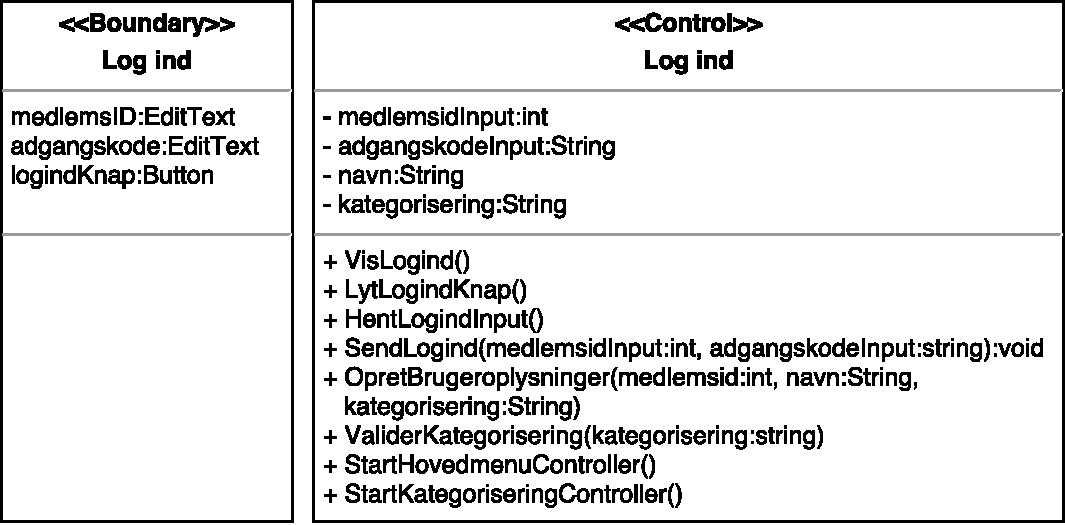
\includegraphics[width=0.7\textwidth]{figures/MVC/MVCLogInd}
\caption{Designklasser for log ind. Til venstre ses grænsefladen og til højre den tilhørende controller.}
\label{fig:Designlogind}
\end{figure}

\noindent
I grænsefladen for \textit{Logind} opstilles tekstfelter af typen EditText, hvor brugeren kan angive medlemsID samt adgangskode. Dertil opsættes en LogindKnap, af typen Button, der ved tryk indikerer, at brugerens informationer er angivet og klar til at logge ind. 

Til denne grænseflade er der opstillet en \textit{Logind} controller. Der er opstillet attributter og metoder af typen private. Disse metoder er Vis, Lyt, Send, Opret, Valider og Start. Controlleren sender log ind i forhold til inputsparametrene, medlemsidInput og adgangskodeInput, hvorefter brugerens oplysninger hentes via controlleren for database. Denne metode fungerer som en void, hvorfor en værdi ikke returneres. Dertil oprettes en entity, brugeroplysninger, hvori oplysninger senere kan lagres. Denne entity beskrives af \autoref{sec:entity}. Ligeledes håndterer controlleren, hvilken grænseflade systemet efterfølgende skal henvises til. Der er i sammenspil med disse designklasser udarbejdet et sekvensdiagram, der fremgår af \autoref{fig:SEKlogind}.


\begin{figure} [H]
\centering
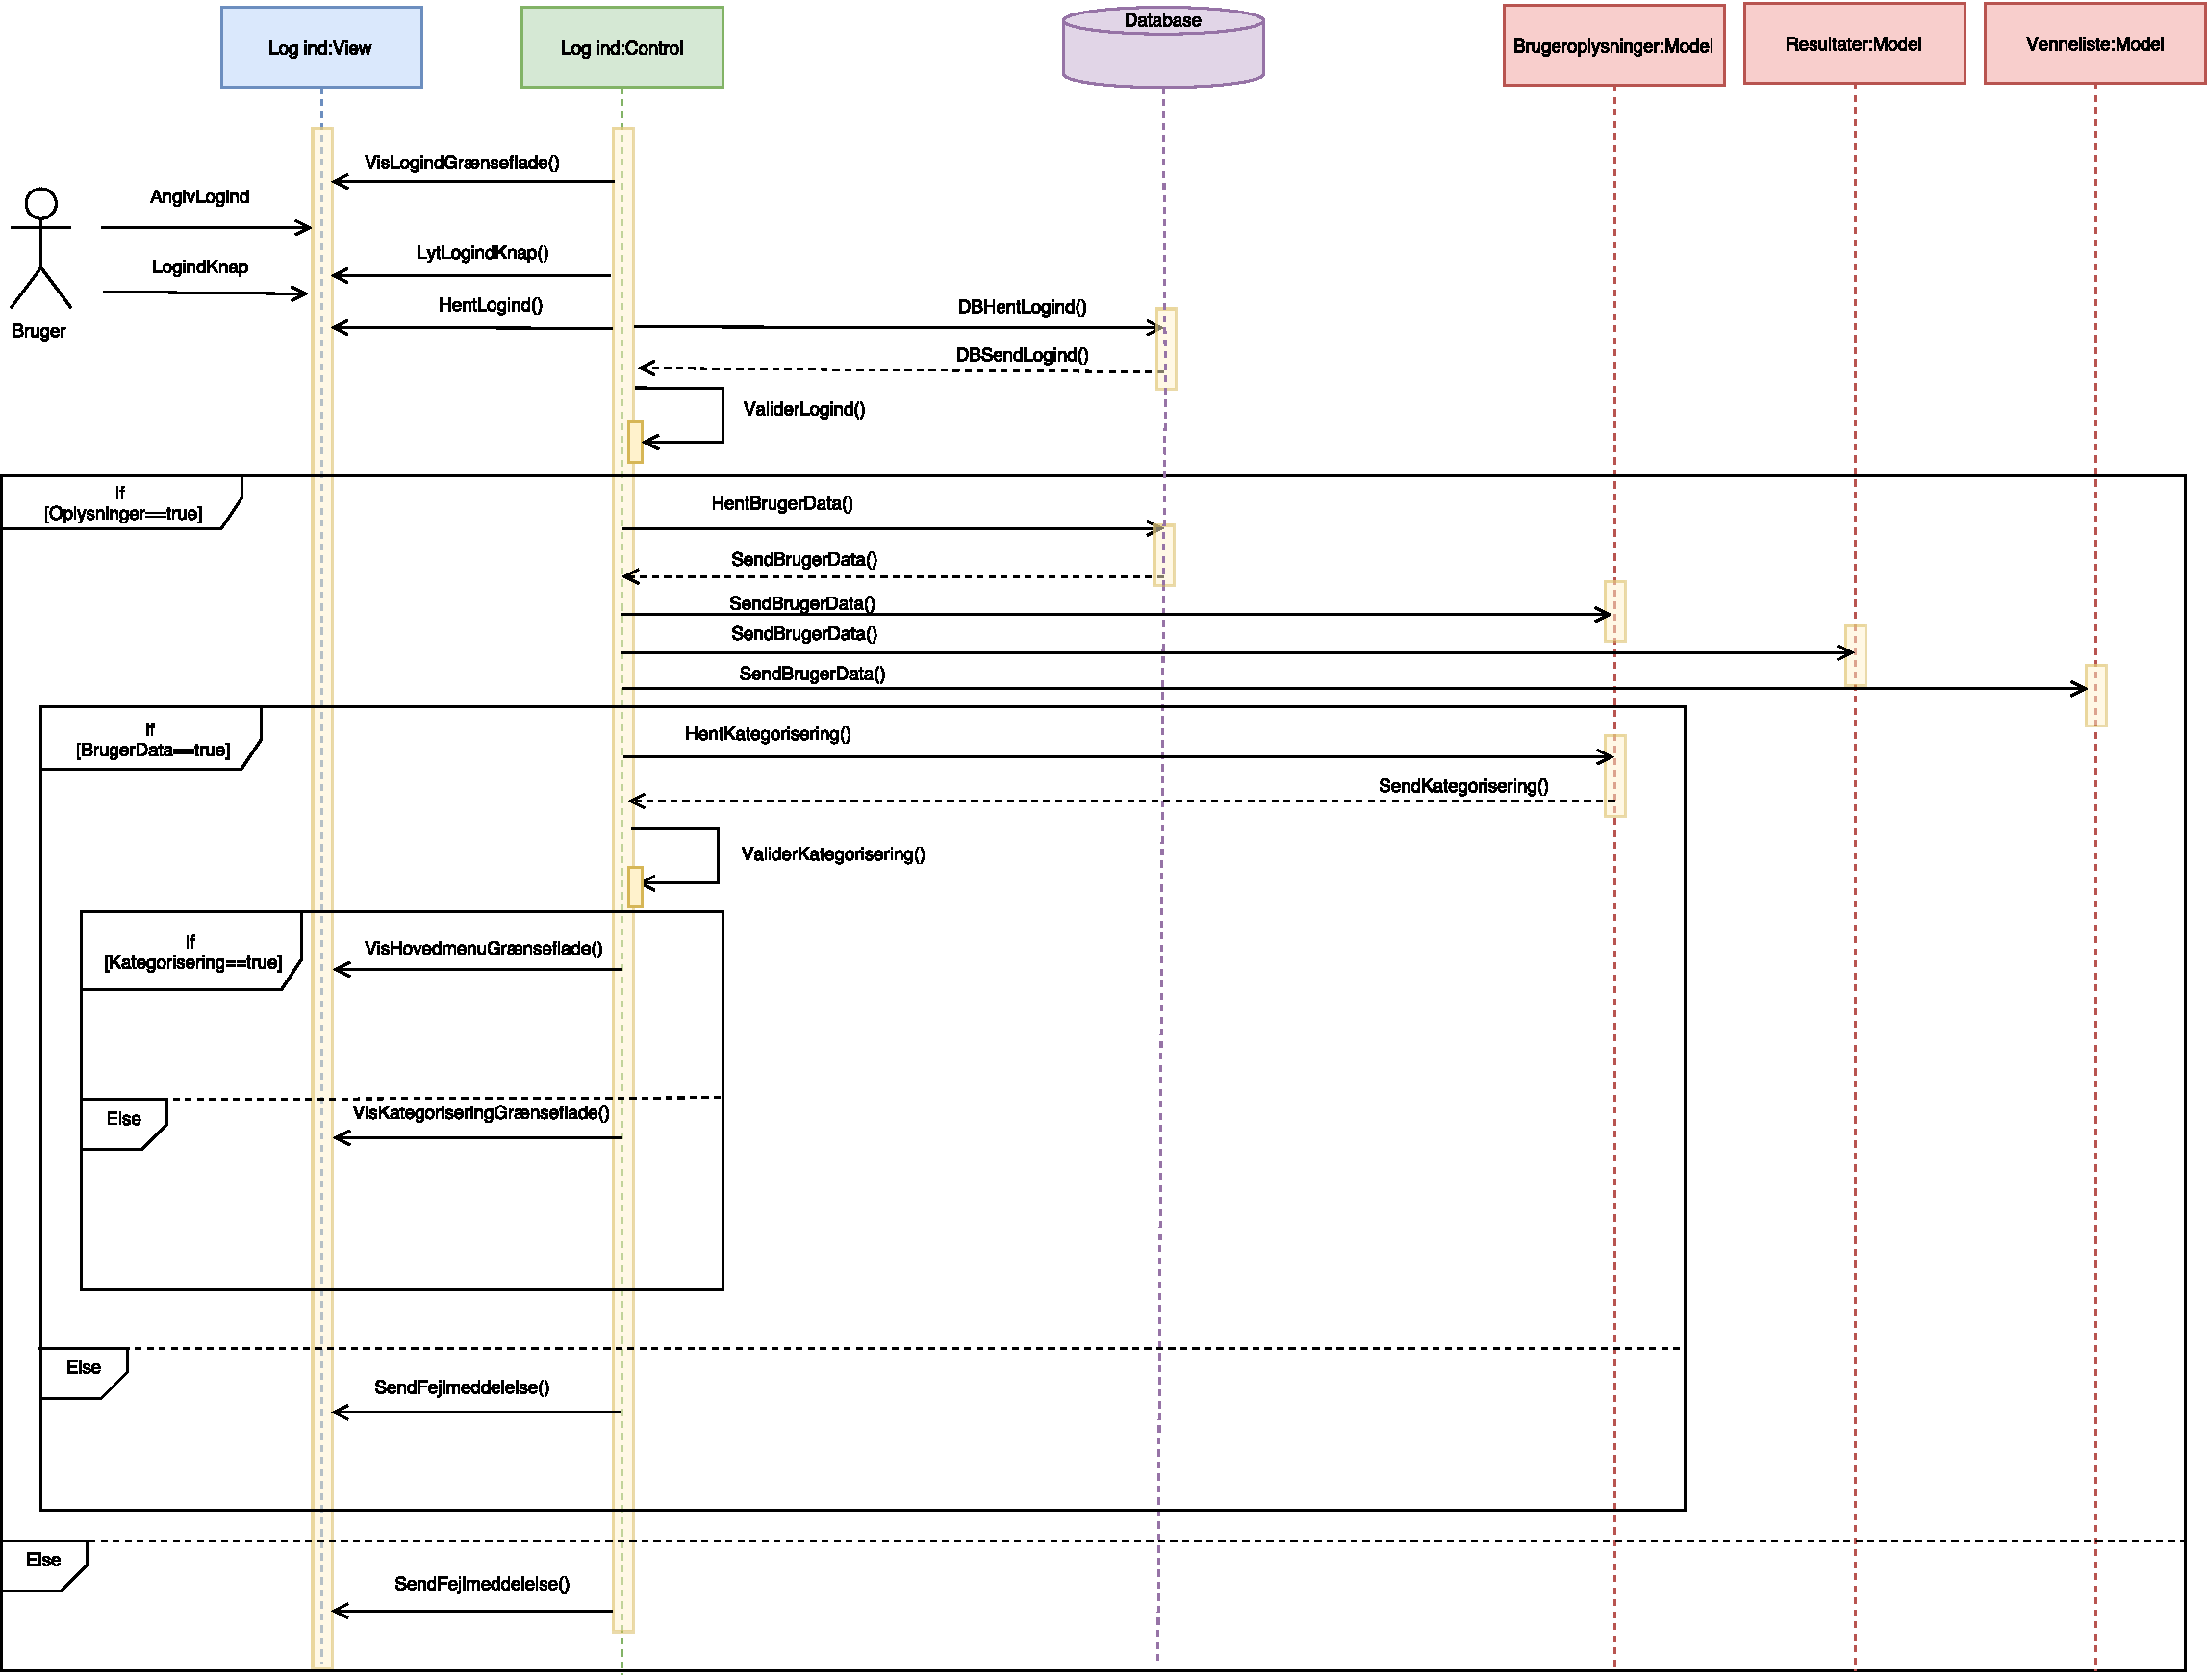
\includegraphics[width=1.55\textwidth, angle=90]{figures/Sek/SEKLogInd}
\caption{Sekvensdiagram for log ind.}
\label{fig:SEKlogind}
\end{figure}

\noindent
Det fremgår af sekvensdiagrammet, at controlleren for \textit{Log ind} starter med at vise grænsefladen for \textit{Log ind}. Dertil lytter controlleren på LogindKnap, der ved tryk henter brugerens angivne log ind-informationer. Dertil sendes disse informationer til \textit{Database} controlleren, der henter brugeren fra databasen og validerer denne. Stjernen definerer inputsparametre, der ses af den tilhørende designklasse for controlleren. 


Bekræftes log ind oprettes en entity af \textit{Brugeroplysninger} med informationerne hentet på brugeren. Herefter validerer \textit{Log ind} controlleren, hvorvidt en kategorisering er foretaget. Forefindes en kategorisering i de hentede brugeroplysninger, startes controlleren for \textit{Hovedmenu}. Eksisterer kategoriseringen ikke, startes \textit{Kategorisering} controlleren. Mislykkes log ind, vises en fejlmeddelelse, der forsvinder efter kort tid, hvorefter brugeren igen har mulighed for at indtaste log ind-oplysninger. 
